\documentclass[../paper.tex]{subfiles}
\begin{document}

\section{Method}

In this section, we describe the technical pipelines of the recognition and production components of our interface. In-depth details on the data collection, model training, and inference stages for the two components are in \autoref{sec:recognition} and \autoref{sec:production}, respectively.

\subsection{Fingerspell Recognition}

Recognition refers to the process of interpreting sign language from a given video or image. In the context of this project, it involves recognizing fingerspelling and translating it into spoken English text. Traditionally, an image classification convolutional neural network (CNN) would be used to recognize fingerspelling. However, with the goal being real-time fingerspell reception in the real world, this component must be fast and accurate, regardless of variability in lighting conditions, backgrounds, skin tones, hand sizes, and distances from the camera. A model trained on images would not be invariant to these factors.

\begin{figure}[!htbp]
  \centerline{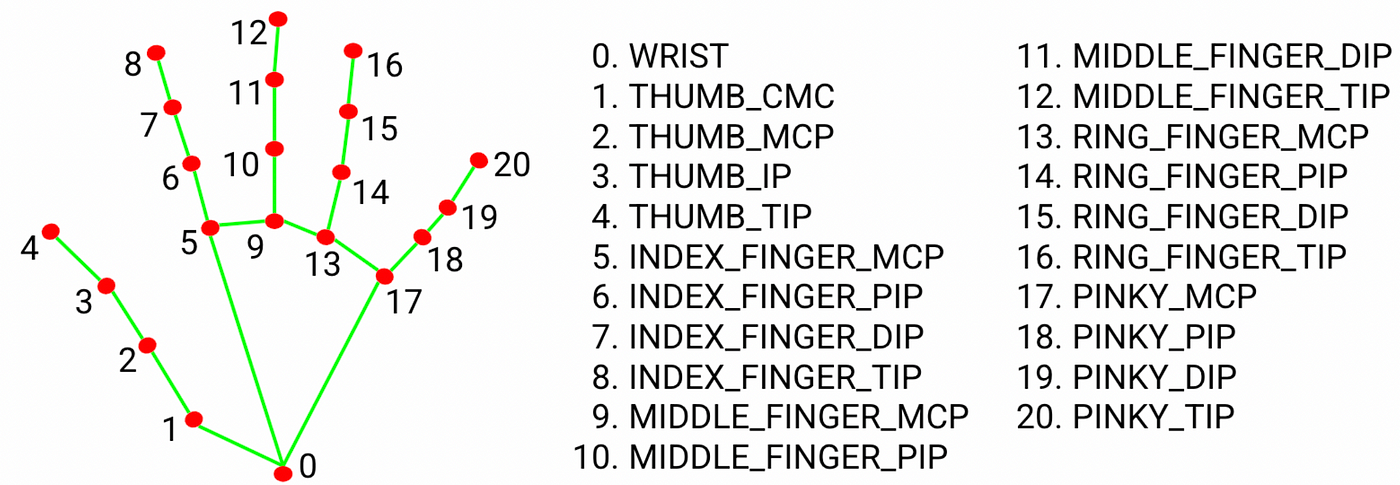
\includegraphics[width=\linewidth]{../figures/mediapipe-hand-landmarks.png}}
  \caption{Google MediaPipe hand landmarks}\label{fig:mediapipe-hand-landmarks}
\end{figure}

To combat this, we used the Google MediaPipe Hand Landmark \cite{MediaPipe} model, allowing for the real-time recognition and pose estimation of hand movements and positions. As seen in \autoref{fig:mediapipe-hand-landmarks}, MediaPipe captures 21 3D landmarks in given images, and it provides detailed information on handedness, hand orientation and finger position of hands in the frame. Furthermore, it can run locally on web browsers and does not require significant computational resources to run in a real-time setting. The use of MediaPipe also allows for the model to be invariant to varying lighting conditions, backgrounds, skin tones, hand sizes, and distances from the camera. By training a model on hand landmarks of fingerspelling images rather than the images themselves, we can achieve a model with low inference time that is invariant to these factors, suitable for real-time fingerspell reception in real-world scenarios.

\subsubsection*{Recognition Pipeline}

\begin{figure}[!htbp]
  \centerline{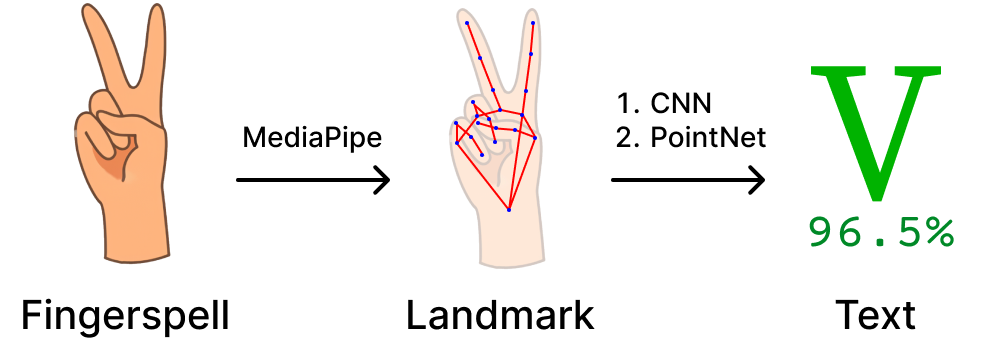
\includegraphics[width=\linewidth]{../figures/recognition-method.png}}
  \caption{Fingerspell recognition pipeline}\label{fig:recognition_method}
\end{figure}

The recognition component must take sequences of frames as input, classify the fingerspelling in each individual frame, and then synthesize the classified English alphabets into spoken English text. For each input frame $\mathbf{F_1, F_2, F_3,...,F_x}$, the model must output the corresponding English alphabet $\mathbf{A_1, A_2, A_3,...,A_y}$. Since a single fingerspelled alphabet can span multiple frames, we can assume $x \geq y$. This process is enabled by a three-step pipeline, as demonstrated in \autoref{fig:recognition_method}: fingerspelling-to-landmark conversion, landmark-to-text classification, and text synthesis.

\subsection{Production}

Sign language production is the process of generating sign language videos from a given text. In the context of this project, production involves translating spoken English text to ASL gloss and generating sequences of animations of the corresponding ASL poses. Traditionally, we would use a simple lookup table to map glosses to poses. However, one of the main challenges in sign language production is the lack of large-scale data sets or sign language corpora. To combat this, we use semantic search to find contextually-similar poses for each gloss, even if the gloss is not present in the data set. This complete sign language production task is enabled by a two-step pipeline, as demonstrated in \autoref{fig:production_method}: text-to-gloss translation and semantic pose retrieval.

\begin{figure}[!htbp]
  \centerline{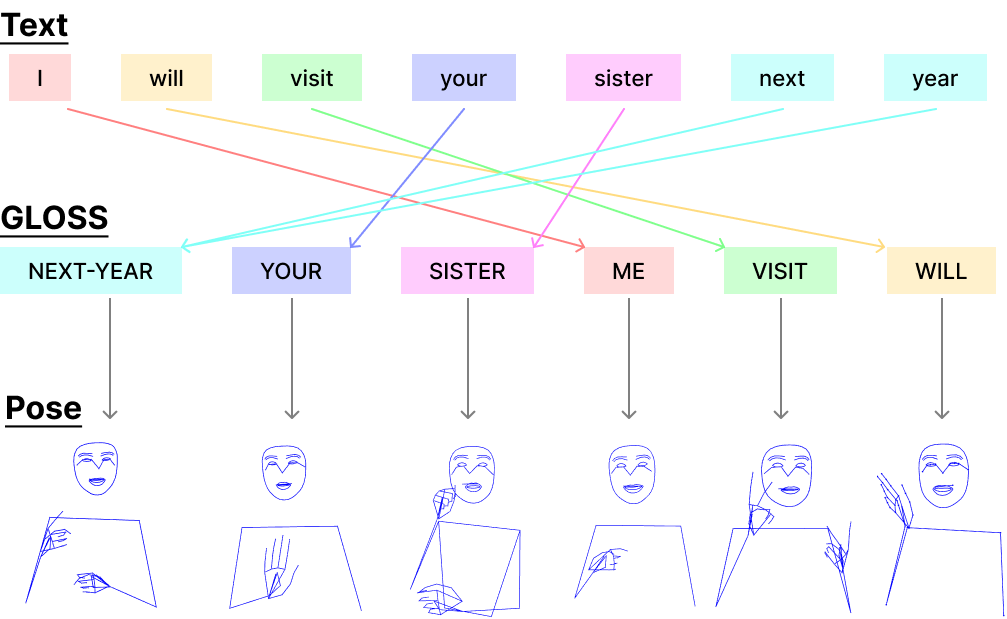
\includegraphics[width=\linewidth]{../figures/production-method.png}}
  \caption{Text \textrightarrow\ Gloss \textrightarrow\ Pose pipeline}\label{fig:production_method}
\end{figure}

\end{document}